\documentclass[a4paper, 12pt]{article}

\usepackage[utf8]{inputenc}
\usepackage[T2A]{fontenc}
\usepackage[english, russian]{babel}

\usepackage{tune}
\usepackage{lipsum}

\def\eng#1{
\unskip
\begin{otherlanguage}{english}
#1
\end{otherlanguage}
}

\def\BR{\mathcal{B}}
\def\Lb{\varLambda_b^0}
\def\Lc{\varLambda_c^+}
\def\Dp{D^+}
\def\Dsp{D^{*+}}
\def\Km{K^-}
\def\pim{\pi^-}
\def\pip{\pi^+}
\def\piz{\pi^0}


\begin{document}

%%%%%%%%%%%%%
%% Heading %%
%%%%%%%%%%%%%
\begin{center}
{\bf Изучение многочастичных распадов $\Lb$ на~Большом адронном коллайдере }

\textit{Гусейнов Абдул-Керим Демирович}\footnote{\mailto{Kerim.Guseinov@cern.ch}}

\textit{МГУ им. М.\,В.~Ломоносова, физический факультет, кафедра общей ядерной физики}
\end{center}

%%%%%%%%%%%%%%%%%%
%% Introduction %%
%%%%%%%%%%%%%%%%%%
\sec{Введение}
Изучение тяжелых барионов и их многочастичных распадов важно для проверки Стандартной модели и поисков новой физики, поскольку в многопетлевых диаграммах Фейнмана возрастает влияние возможных новых частиц. 
$\Lb$ -- самый легкий прелестный барион, его распады с переходом барионного числа протону интересны еще и для изучения адронизации кварков. 
При изучении распадов по спектру инвариантных масс важную роль играет модель соответствующих вкладов в спектр. В зависимости от нее, конечный результат может иметь разную систематическую погрешность, быть более или менее стабильным по отношению к статистическим погрешностям экспериментальных данных.

\begin{figure}[b]
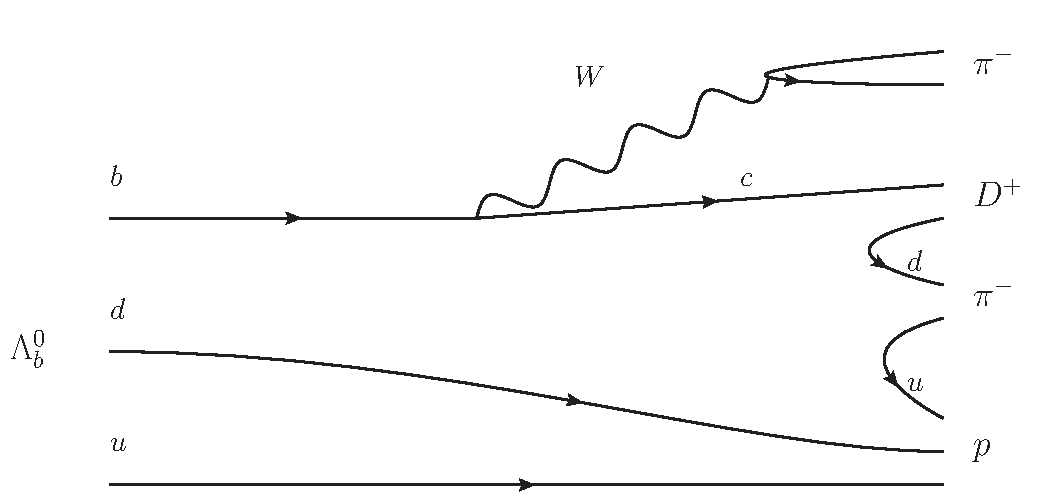
\includegraphics[width=.6\linewidth]{figures/Feynman}
\caption{Диаграмма Фейнмана, дающая вклад в распад $\Lb\to\Dp p\pim\pim$.}
\label{fig:Feynman}
\end{figure}

В работе рассматриваются многочастичные распады $\Lb\to\Dp p\pim\pim$ и $\Lb\to\Dsp p\pim\pim$, одна из диаграмм Фейнмана для которых изображена на рисунке~\ref{fig:Feynman}. 
Основная цель -- измерение вероятностей названных каналов распада $\Lb$. 
Для этого продукты распадов регистрируются в следующих модах: $\Dp\to\Km\pip\pip$, $\Dsp\to\Dp\piz$ или $\Dp\gamma$. 
Нейтральные частицы не восстанавливаются, оба распада $\Lb$ изучаются по спектру инвариантных масс $\Dp p \pim\pim$. 
Для смягчения влияния различных неопределенностей из-за геометрии детектора и эффективностей регистрации частиц и получения более точного результата искомые вероятности распадов вычисляются в отношении к уже изученной вероятности канала $\Lb\to\Lc\pip\pim\pim$~\cite{LbLc_LHCb, LbLc_CDF}.
$\Lc$ регистрируется в моде $\Lc\to p\Km\pip$. 
При таком выборе и изучаемый, и нормировочный распады имеют один и тот же набор конечных частиц. 
Это несколько усложняет обработку и заставляет учитывать перекрестные вклады, но существенно подавляет систематические погрешности.

В итоге изучаются отношения 
\[ R = \frac{\BR(\Lb\to\Dp p \pim\pim)}{\BR(\Lb\to\Lc\pip\pim\pim)} 
  \times \frac{\BR(\Dp\to\Km\pip\pip)}{\BR(\Lc\to p\Km\pip)} , \]
\[ R^* = \frac{\BR(\Lb\to\Dsp p\pim\pim)}{\BR(\Lb\to\Dp p\pim\pim)} 
  \times {\BR(\Dsp\to\Dp\piz \text{ или } \Dp\gamma)}  . \]
Далее распад $\Lb\to\Dp p\pim\pim$ будет называться основным сигналом, $\Lb\to\Dsp p\pim\pim$~-- резонансным сигналом, а $\Lb\to\Lc\pip\pim\pim$~-- нормировочным сигналом. 

\sec{Модель}
Рассмотрим спектр инвариантных масс $\Dp p\pim\pim$ в интересующем нас диапазоне, вблизи $M(\Lb) \sim 5620$ МэВ$/c^2$~\cite{PDG}.
В нем присутствуют вклады четырех распадов: $\Lb\to\Dp p\pim\pim$, $\Lb\to\Dsp p\pim\pim$ ($\Dsp\to\Dp\piz/\gamma$), $\Lb\to\Dp\piz p\pim\pim$ и комбинаторный фон. Последний можно аппроксимировать, например, полиномом третьей степени. 

Так как в основном сигнале все частицы заряженные и успешно восстанавливаются, его вклад в спектр масс достаточно узкий, и мы можем выбрать шаблонную аппроксимирующую функцию.
Поскольку хвосты отклика детектора не описываются функцией Гаусса, а также частицы в детекторе теряют энергию, что также не подчиняется распределению Гаусса, необходимо учесть несовпадение формы вклада основного сигнала с гауссианом. 
Для этого была выбрана следующая функция: 
\begin{equation}
S_{\Dp} = N\cdot
\begin{cases}
\exp\left(-\frac{(m-m_0)^2}{2\sigma_m^2}\right), & -\alpha_L < \frac{m-m_0}{\sigma_m} < \alpha_R, \\
A_L\cdot\left(B_L - \frac{m-m_0}{\sigma_m}\right)^{-n_L}, & \frac{m-m_0}{\sigma_m} \leq -\alpha_L, \\
A_R\cdot\left(B_R + \frac{m-m_0}{\sigma_m}\right)^{-n_R}, & \frac{m-m_0}{\sigma_m} \geq \alpha_R, 
\end{cases}
\label{eq:S1}
\end{equation}
в которой $m = m(\Dp p\pim\pim)$; $\alpha_L$, $\alpha_R$, $n_L$, $n_R$, $m_0$, $\sigma_m$ -- параметры аппроксимации, каждый из которых больше нуля, а $n_L,\,n_R>1$. 
Коэффициенты $A_L$, $A_R$, $B_L$, $B_R$, $N$ находятся из условий нормировки $S_{\Dp}$ на единицу и непрерывности $S_{\Dp}(m)$ и ее производной. 
Функция такого вида была впервые рассмотрена участником коллаборации Crystal Ball~\cite{CrystalBallFunction} и называется Crystal Ball функцией. 
Ее сравнение с традиционным распределением Гаусса от переменной $x=\frac{m-m_0}{\sigma_m}$ для иллюстративного набора параметров показано на рисунке~\ref{fig:CrystalBall}.

\begin{figure} %
\begin{minipage}{.48\linewidth} %
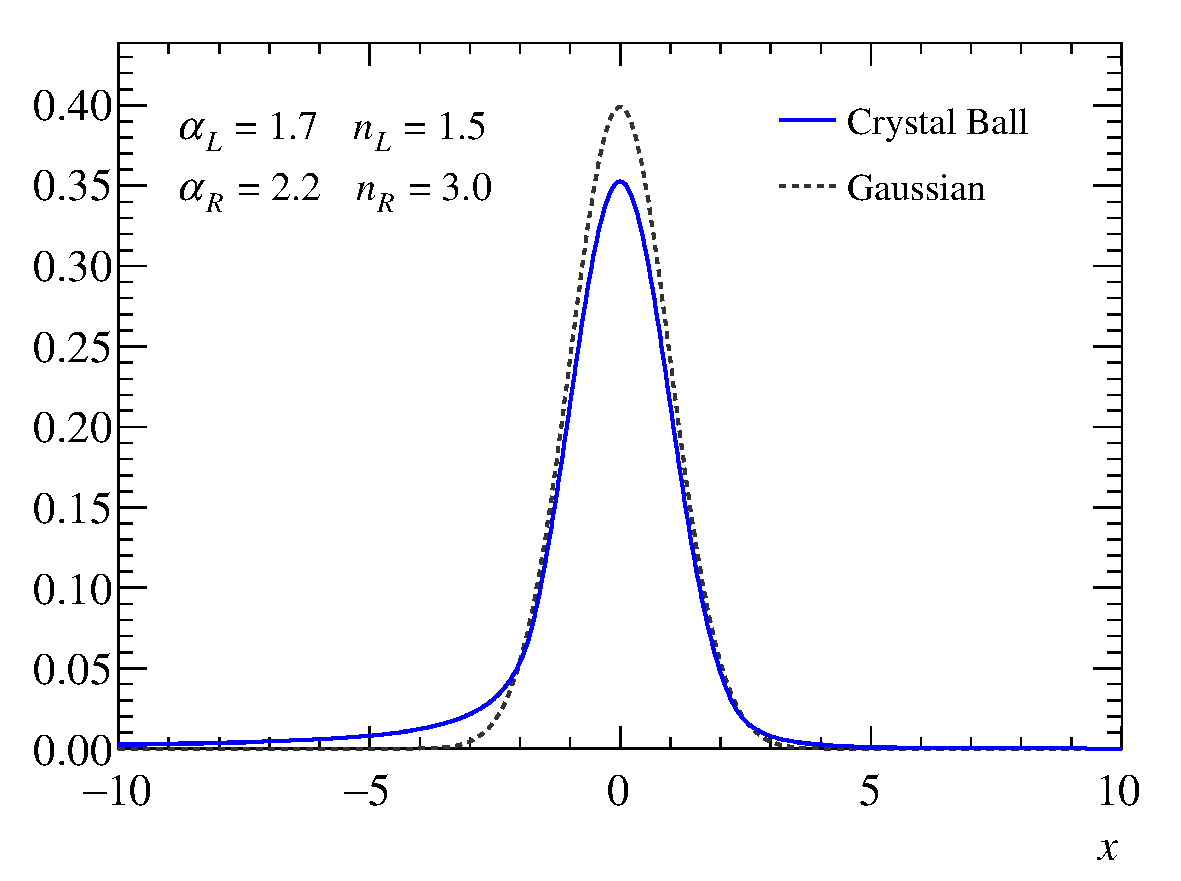
\includegraphics[width=\linewidth]{figures/CrystalBall}
\captionof{figure}{Сравнение выбранной модели основного сигнала с функцией Гаусса.}
\label{fig:CrystalBall}
\end{minipage} 
\hfill
\begin{minipage}{.48\linewidth} %
\vskip5ex\null\hspace*{-4ex}
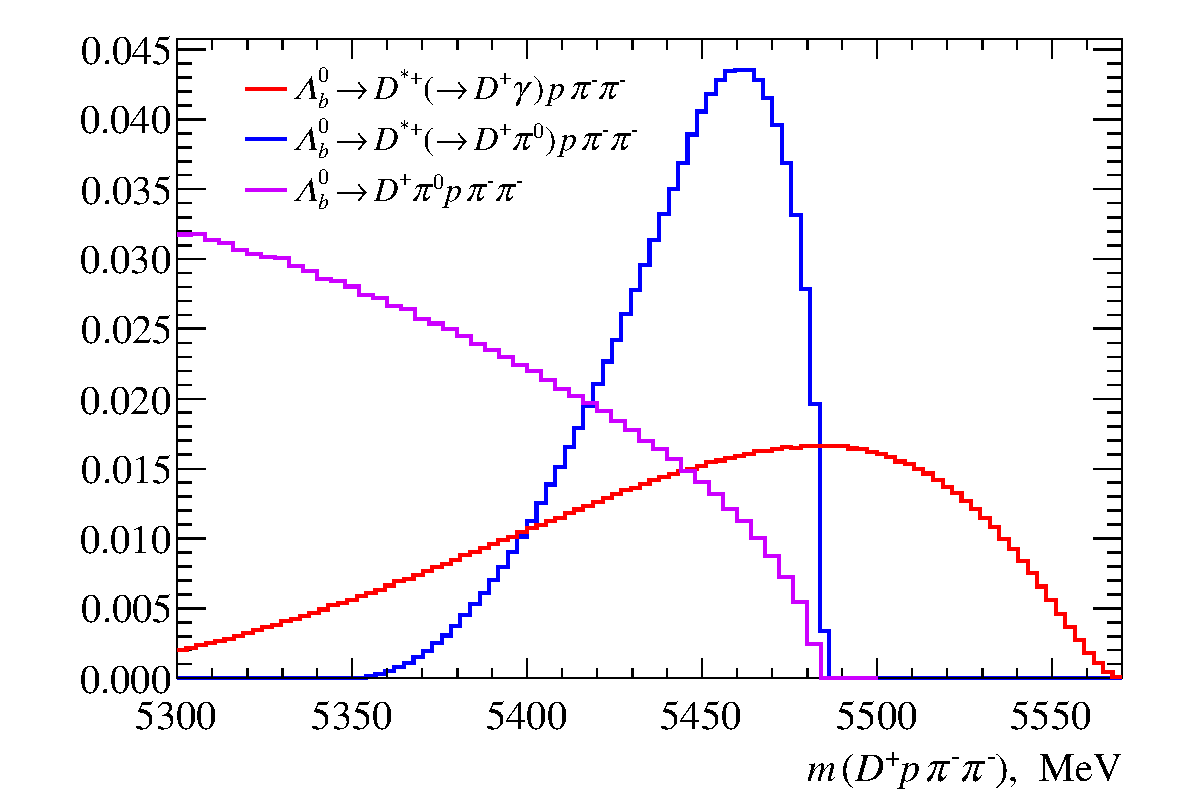
\includegraphics[width=1.1\linewidth]{figures/Neutral_particles}
\captionof{figure}{Монте-Карло моделирование распределений инвариантной массы $\Dp p\pim\pim$ распадов с нейтральными частицами.}
\label{fig:neutral}
\end{minipage} %
\end{figure}

Для распадов с образованием дополнительных нейтральных частиц на форму вклада сильно влияет кинематика. 
В связи с этим, каждый распад моделируется методом Монте-Карло, и определяются вклады в спектр инвариантных масс $m(\Dp p\pim\pim)$. Результаты моделирования представлены на рисунке~\ref{fig:neutral}.
После этого нужно учесть отклик детектора, свернув полученные распределения с гауссианом с нулевым средним и конечной шириной. 
Кроме того, вероятности распадов $\Dsp\to\Dp\piz$ и $\Dsp\to\Dp\gamma$ равны $30.7\pm0.5$\% и $1.6\pm0.4$\% соответственно~\cite{PDG},  
поэтому при попытках независимо определить величины их вкладов из экспериментального спектра будут возникать большие ошибки, аппроксимация не окажется устойчивой. 
Чтобы этого избежать, необходимо использовать сумму этих вкладов с коэффициентами, соответствующими названным вероятностям. 
%В результате определяются вклады $S_{\Dsp}$ распадов с участием $\Dsp$ и $S_{\Dp\piz}$ распада $\Lb\to\Dp\piz p\pim\pim$. 

Полная функция распределения представляет собой сумму четырех перечисленных компонент с коэффициентами, выражающими числа событий в каждом канале. 
Для определения всех параметров модели ищется максимум функции правдоподобия. 
Поскольку величины экспериментальных сигналов сравнительно небольшие, при их аппроксимации параметры степенных хвостов функции $S_{\Dp}$ фиксируются на значениях, полученных из данных Монте-Карло моделирования. 

Спектр инвариантных масс $\Lc\pip\pim\pim$ имеет аналогичную структуру, создаваемую распадами $\Lb\to\Lc\pip\pim\pim$, $\Lb\to\varSigma_c^+\pip\pim\pim$ ($\varSigma_c^+\to\Lc\piz$), $\Lb\to\Lc\piz\pip\pim\pim$. 
Аппроксимирующая функция строится так же, как и для спектра $m(\Dp p\pim\pim)$.

\sec{Систематические погрешности модели}
Выбор модели может оказывать различное влияние на результат аппроксимации. 
При достаточно удачном выборе, учитывающем физические особенности распадов и вместе с ними распределений по инвариантным массам, зависимость результата от параметров, на которые полагается модель, будет слабой. 
Вносимую моделью погрешность можно оценить, варьируя такие параметры модели в соответствующих им пределах. 

Для вклада основного сигнала варьируются величины параметров хвостов \eng{Crystal Ball} функции в пределах погрешностей, полученных при аппроксимации данных Монте-Карло. 
Для комбинаторного фона изменяется вид функции: рассматривается полином второй степени, произведение полинома и убывающей экспоненты. 
Для резонансного сигнала, как уже обсуждалось, необходимо пользоваться моделью, представляющей из себя сумму вкладов с распадами $\Dsp\to\Dp\piz$ и $\Dsp\to\Dp\gamma$. 
Однако вероятности этих распадов известны с конечной точностью, поэтому коэффициенты при их вкладах не определены строго. 
При изменении отношения коэффициентов в пределах его погрешности будет меняться модель резонансного сигнала. 
Как видно из рисунка~\ref{fig:neutral_syst}, это изменение мало, и связанная с ним систематическая погрешность невелика.

Так как модель нормировочного канала практически целиком повторяет модель изучаемого, вносимые ей систематические погрешности аналогичны. 


\begin{figure}
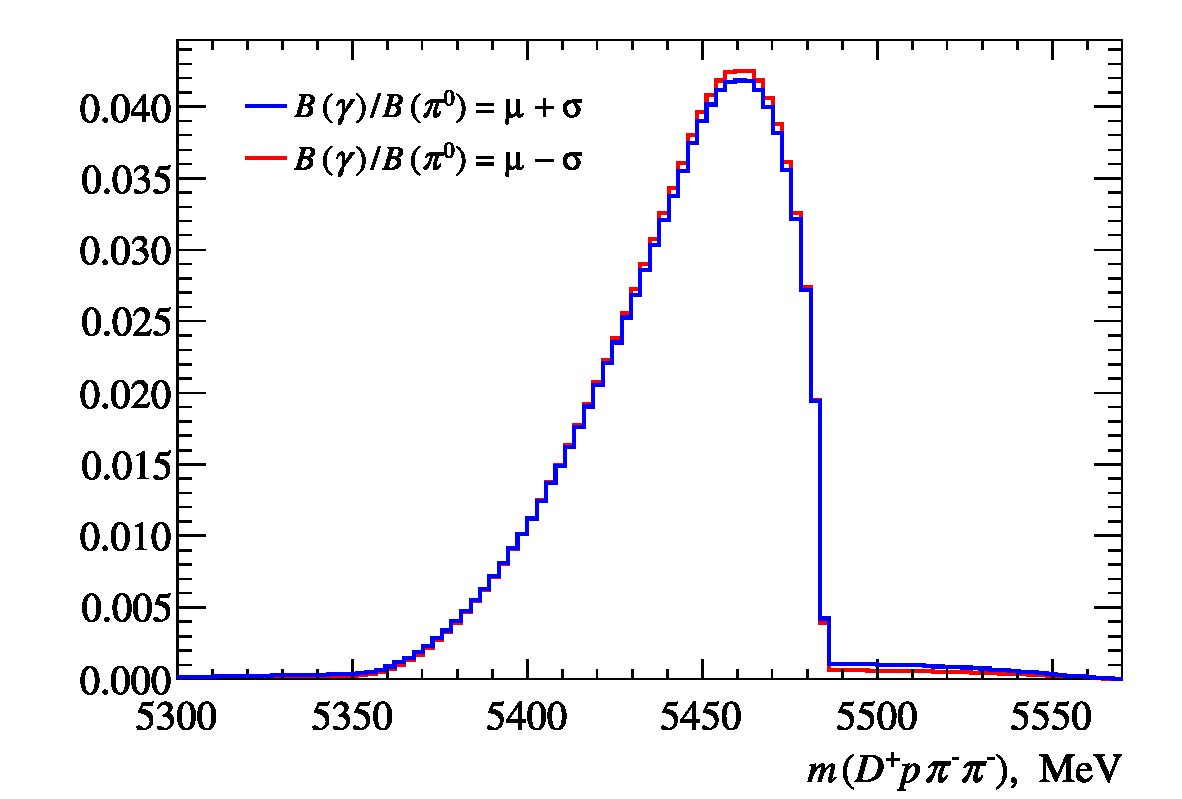
\includegraphics[width=.5\linewidth]{figures/Neutral_particles_syst}
\caption{Изменение модели резонансного сигнала при вариации коэффициентов суммирования вкладов $\Dsp\to\Dp\piz$ и $\Dsp\to\Dp\gamma$.}
\label{fig:neutral_syst}
\end{figure}


\sec{Стабильность аппроксимации}
Алгоритм минимизации для каждого параметра модели находит центральное значение и погрешность. 
В некоторых случаях, чаще со сложными моделями, найденные алгоритмом значения могут отличаться от истинных результатов. 
Для проверки истинности найденных результатов и стабильности аппроксимации вблизи полученных значений параметров необходимо проводить дополнительный анализ. 

Поскольку экспериментальные данные -- случайные числа, а искомые параметры модели -- их функции, то значения параметров тоже являются случайными. 
Это значит, что исследовать любые их свойства следует статистическими методами. 
То есть требуется многократно проводить одну и ту же процедуру аппроксимации одной и той же модели, но с разными аппроксимируемыми данными, отличающимися друг от друга в пределах статистических погрешностей. 
Для получения таких наборов данных можно воспользоваться генераторами псевдослучайных чисел, генерируя значения случайной величины, распределенной согласно модели. 

\begin{figure}
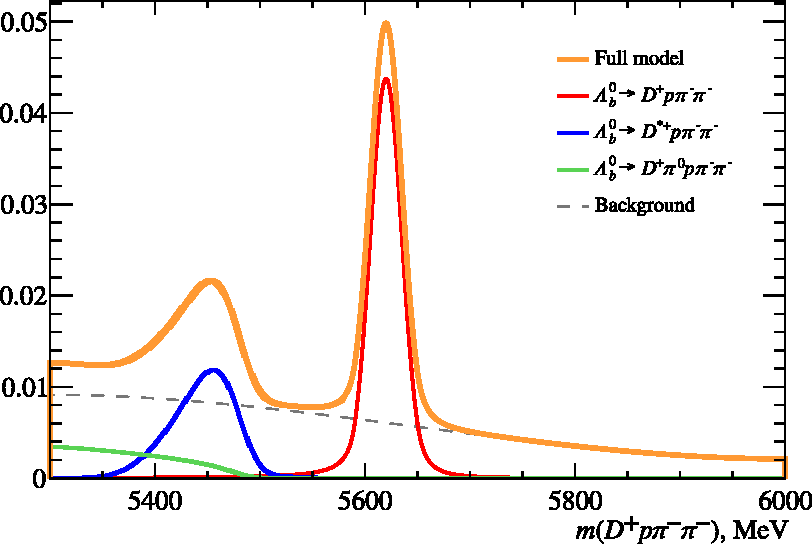
\includegraphics[width=.5\linewidth]{figures/model_plot}
\caption{Форма модели для составленного набора значений параметров.}
\label{fig:model}
\end{figure}

\begin{figure}[b]
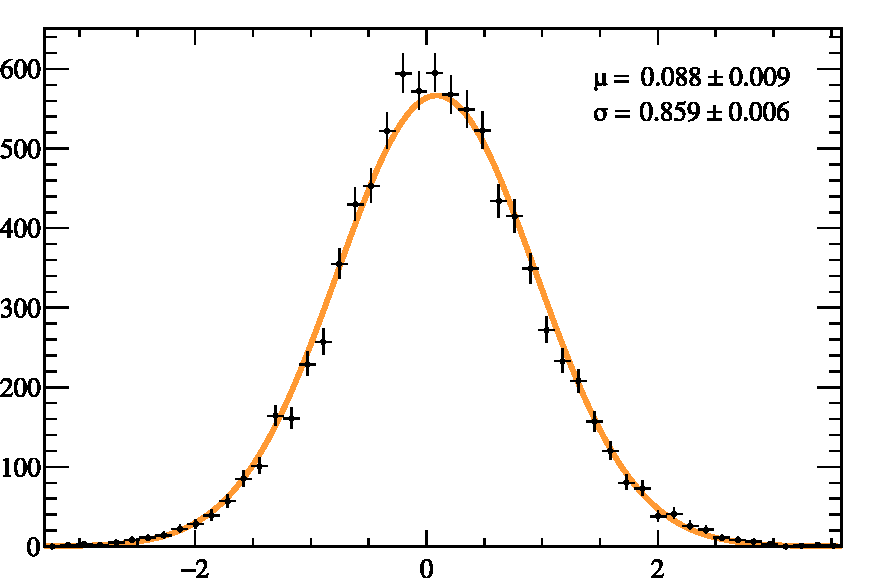
\includegraphics[width=.32\linewidth]{figures/toy_signal}
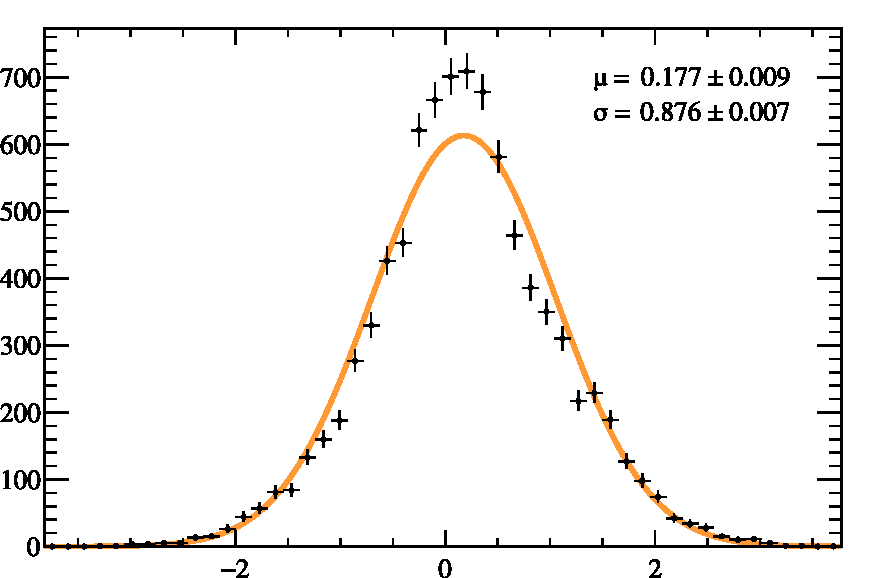
\includegraphics[width=.32\linewidth]{figures/toy_star}
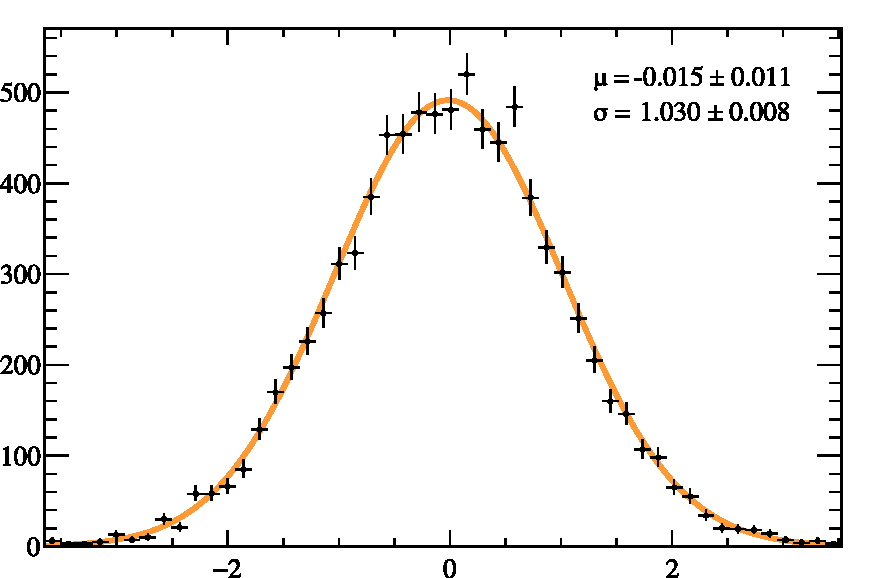
\includegraphics[width=.32\linewidth]{figures/toy_mass}
\caption{Полученные при изучении свойств алгоритма минимизации распределения числа событий в сигнальном канале (слева), в резонансном канале (в центре) и массы (справа).}
\label{fig:toys}
\end{figure}

Для исследования свойств алгоритма минимизации в условиях, похожих на реальные, был составлен набор значений параметров модели, основанный на~\cite{LbLc_LHCb} и~\cite{PDG}. 
На основе этой модели генерировались спектры инвариантных масс $\Dp p\pim\pim$, а затем аппроксимировались ей же. 
Для каждого параметра~$p_i$ результат аппроксимации~$p^\mathrm{fit}_i$ записывался в форме нормированного на найденную погрешность~$\sigma^\mathrm{fit}_i$ отклонения от исходного значения~$p^\mathrm{orig}_i$, с которым генерировался спектр: 
\[ x_i = \frac{p^\mathrm{fit}_i - p^\mathrm{orig}_i}{\sigma^\mathrm{fit}_i}. \]
Набиралось статистически значимое количество результатов аппроксимации, а затем изучались полученные распределения $x_i$. 
В идеальном случае, когда алгоритм правильно находит и центральные значения, и погрешности, эти распределения должны представлять собой гауссианы с нулевым средним~$\mu_i$ и единичной дисперсией~$\sigma^2_i$. 
Если же среднее или дисперсия отличаются от идеальных значений, определяемый алгоритмом результат необходимо поправлять: сместить центральное значение и изменить ошибку. Если изначальный результат для параметра~$p_i$ был~$p^\mathrm{init}_i$ и~$\sigma^\mathrm{init}_i$, то откорректированный результат определяется по формулам
$$ p_i^\mathrm{corr} = p^\mathrm{init}_i + \mu_i\,\sigma_i\,\sigma^\mathrm{init}_i,
\qquad
\sigma_i^\mathrm{corr} = \sigma_i\,\sigma^\mathrm{init}_i. $$

Для составленной модели были изучены свойства стандартного алгоритма минимизации Minuit2 программного пакета ROOT. Распределения чисел событий в разных каналах, как наиболее важных результатов, а также массы $\Lb$, как наиболее точного результата, показаны на рисунке~\ref{fig:toys}. 


\sec{Заключение}
Рассмотрены вклады в спектр инвариантных масс $\Dp p\pim\pim$ вблизи массы $\Lb$-бариона, для каждого из них построена модель. 
Изучены свойства выбранных моделей и эффективность их использования с алгоритмом минимизации Minuit2. 
Установлено, что результаты аппроксимации этой моделью устойчивы, и модель не вносит большой систематической погрешности, а также, что
поведение модели при использовании Minuit2 не идеально, но в достаточной мере точно и предсказуемо. 








%%%%%%%%%%%%%%%%%%
%% Bibliography %%
%%%%%%%%%%%%%%%%%%
\bibliographystyle{local}
\bibliography{Refs.bib}

\end{document}
